\documentclass{article}
\usepackage[utf8]{inputenc}
\usepackage{cite}
\usepackage{graphicx}
\usepackage{svg}

\title{GDMA Project: \\ CDDB as Graph Database}
\author{Julian Schelb (1069967)}
\date{June 2022}

\begin{document}

\maketitle

\section{Importing Data}

In the following, some design decisions are described, made when converting the relational database to a graph.



\begin{figure}[ht]
    \centering
    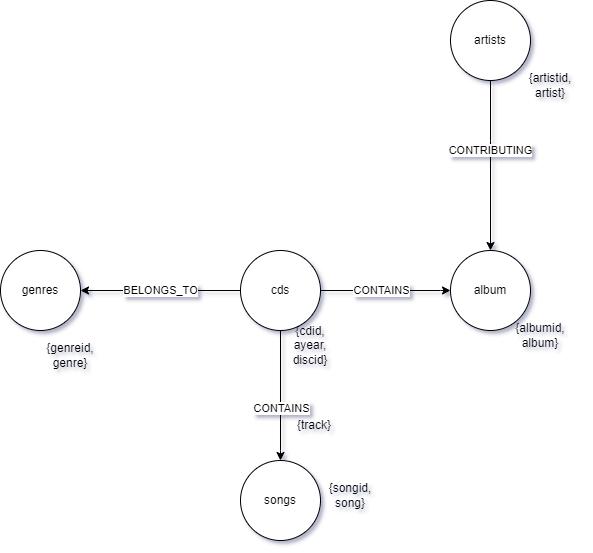
\includegraphics[width=11.5cm]{../Figures/cddb_as_graph-Default.png}
    \caption{CDDB Graph Schema }
\end{figure}



% \begin{figure}
%     \centering
%     \includesvg{../Figures/cddb_as_graph.svg}
%     \caption{svg image}
% \end{figure}

\vspace*{2mm}
\noindent
\textbf{Mappping of tables:} Entries in the tables "artist", "albums", "songs" and "cds" represent entities and are mapped to nodes of appropriate type. The cross table "cdtracks" is mapped as relations between CDs and Songs with the property "track". The cross table "artist2album" is mapped as "triangular relationships", using six relations each to connect Artists, Albums and CDs in both directions.

\vspace*{2mm}
\noindent
\textbf{Bidirectional relations:} For the subsequent queries, it was not necessary to create relations for both directions. However, some queries can be implemented in a more readable manner this way. In addition, the relational SQL database does not define a direction for relations, and this property is thereby preserved.

\vspace*{2mm}
\noindent
\textbf{IDs:} The unique identifiers were preserved as node properties. Although Neo4J automatically assigns different IDs internally, this preserves compatibility  with the SQL version. It is conceivable that for some usecases queries directly utilize these IDs. For example they may be hardcoded as part of a GUI.

\vspace*{2mm}
\noindent
\textbf{Names:} As in the SQL version, the actual name of a song, genre, album and artist is a property named like the entity type and therefore different for nodes of different node labels. This was done to map the SQL version as closely as possible to the graph version. It might be a good idea to rename these properties to "name". This would allow for easier queries when filtering among multiple node names is required. It would also be possible to create a joint full-text index.

\vspace*{2mm}
\noindent
\textbf{Indices:} To speed up "MERGE" and "MATCH" operations, the IDs for nodes of labels "Artist", "Album", "Genre", "Song" and "CD" are indexed. In addition, a full text index is used for "Artists", "Albums" and "Songs" to allow for imprecise searches.

Lorem Ipsum ... ~\cite{Nobody06}.

\section{Cypher Queries}

\section{SQL to Cypher}

\section{Searching and Ranking}

\bibliography{references}{}
\bibliographystyle{plain}
\end{document}
